\documentclass{paper}

%\usepackage{times}
\usepackage{epsfig}
\usepackage{graphicx}
\usepackage{amsmath}
\usepackage{amssymb}
\usepackage{color}
\usepackage{caption}
\usepackage{subcaption}


% load package with ``framed'' and ``numbered'' option.
%\usepackage[framed,numbered,autolinebreaks,useliterate]{mcode}

% something NOT relevant to the usage of the package.
\setlength{\parindent}{0pt}
\setlength{\parskip}{18pt}
\graphicspath{{images/}}


\usepackage[latin1]{inputenc}
\usepackage[T1]{fontenc}


\usepackage{listings}
\lstset{%
   language=R,
   basicstyle=\small\ttfamily,
   frame=single
}



\title{Assignment 5}



\author{Jenni Simon\\09-116-005}
% //////////////////////////////////////////////////


\begin{document}



\maketitle


% Add figures:
%\begin{figure}[t]
%%\begin{center}
%\quad\quad   \includegraphics[width=1\linewidth]{ass2}
%%\end{center}
%
%\label{fig:performance}
%\end{figure}


\paragraph{Exercise 1}

Figure \ref{fig:res1} and listing \ref{list:res1} show results for the multiple
linear regression model with target variable 'Wage'.



\begin{figure}
  \begin{center}
    \quad\quad
    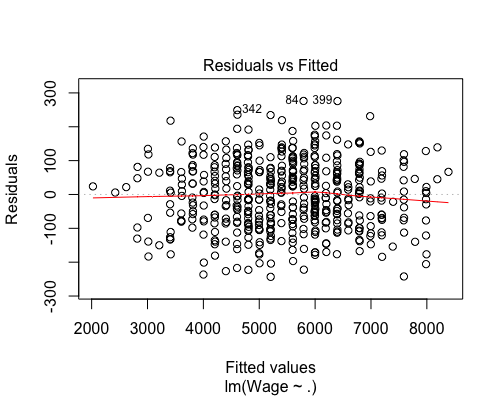
\includegraphics[width=.8\linewidth]{res1}
  \end{center}
  \caption{Plot showing the residuals against the fit of the multiple regression
   model of exercise 1.}
   \label{fig:res1}
\end{figure}

\begin{figure}
  \begin{center}
    \quad\quad
    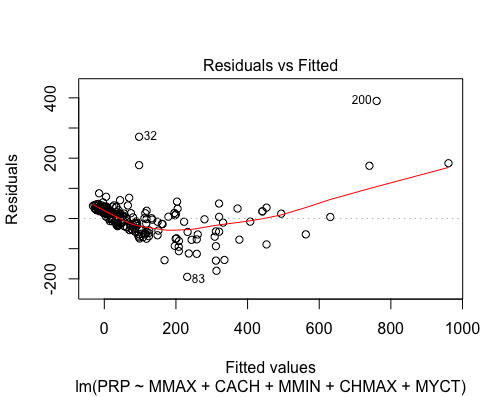
\includegraphics[width=.8\linewidth]{res2}
  \end{center}
  \caption{Plot showing the residuals against the fit of the multiple regression
   model of exercise 2.}
   \label{fig:res2}
\end{figure}

\begin{figure}
  \begin{center}
    \quad\quad
    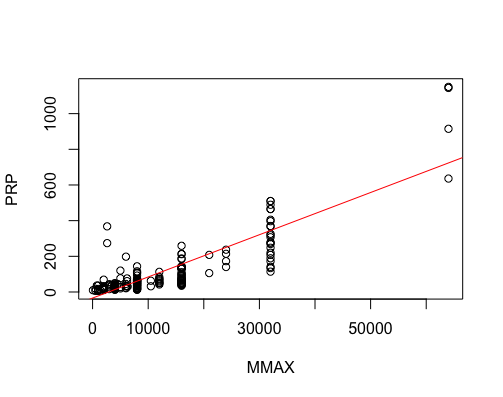
\includegraphics[width=.8\linewidth]{ex3}
  \end{center}
  \caption{Plot showing the linear regression
   model of exercise 3.}
   \label{fig:ex3}
\end{figure}

\begin{figure}
  \begin{center}
    \quad\quad
    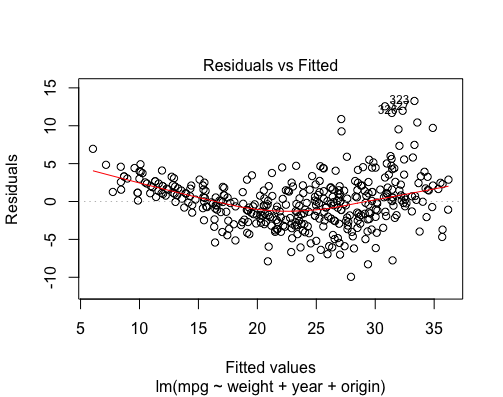
\includegraphics[width=.8\linewidth]{res4}
  \end{center}
  \caption{Plot showing the residuals against the fit of the multiple regression
   model of exercise 4.}
   \label{fig:res4}
\end{figure}

\begin{figure}
  \begin{center}
    \quad\quad
    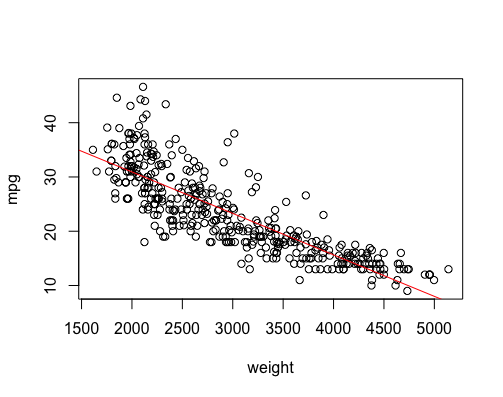
\includegraphics[width=.8\linewidth]{ex4}
  \end{center}
  \caption{Plot showing the linear regression
   model of exercise 4.}
   \label{fig:ex4}
\end{figure}

\begin{minipage}{\linewidth}
  \begin{lstlisting}[caption={Summary of multiple regression fit for exercise 1},
    label=list:res1]

Residuals:
     Min       1Q   Median       3Q      Max
-243.334  -75.119    2.669   70.007  276.238

Coefficients:
              Estimate Std. Error t value Pr(>|t|)
(Intercept) -576.22317   24.08079 -23.929   <2e-16 ***
ID             0.02952    0.03114   0.948    0.344
Education    397.90661    1.54440 257.645   <2e-16 ***
Gendermale   597.94707    9.17422  65.177   <2e-16 ***
---

Residual standard error: 100.1 on 493 degrees of freedom
Multiple R-squared:  0.9931,	Adjusted R-squared:  0.9931
F-statistic: 2.362e+04 on 3 and 493 DF,  p-value: < 2.2e-16

  \end{lstlisting}
\end{minipage}


\begin{minipage}{\linewidth}
  \begin{lstlisting}[caption={Summary of multiple regression fit for exercise 2},
    label=list:res2]

Residuals:
    Min      1Q  Median      3Q     Max
-193.37  -24.95    5.76   26.64  389.66

Coefficients:
              Estimate Std. Error t value Pr(>|t|)
(Intercept) -5.608e+01  8.007e+00  -7.003 3.59e-11 ***
MMAX         5.562e-03  6.396e-04   8.695 1.18e-15 ***
CACH         6.298e-01  1.344e-01   4.687 5.07e-06 ***
MMIN         1.518e-02  1.788e-03   8.490 4.34e-15 ***
CHMAX        1.460e+00  2.076e-01   7.031 3.06e-11 ***
MYCT         4.911e-02  1.746e-02   2.813   0.0054 **
---

Residual standard error: 59.86 on 203 degrees of freedom
Multiple R-squared:  0.8648,	Adjusted R-squared:  0.8615
F-statistic: 259.7 on 5 and 203 DF,  p-value: < 2.2e-16

  \end{lstlisting}
\end{minipage}


\begin{minipage}{\linewidth}
  \begin{lstlisting}[caption={Summary of multiple regression fit for exercise 4},
    label=list:res3]

Residuals:
    Min      1Q  Median      3Q     Max
-9.9440 -2.0948 -0.0389  1.7255 13.2722

Coefficients:
              Estimate Std. Error t value Pr(>|t|)
(Intercept) -1.805e+01  4.001e+00  -4.510 8.60e-06 ***
weight      -5.994e-03  2.541e-04 -23.588  < 2e-16 ***
year         7.571e-01  4.832e-02  15.668  < 2e-16 ***
origin       1.150e+00  2.591e-01   4.439 1.18e-05 ***
---

Residual standard error: 3.348 on 388 degrees of freedom
Multiple R-squared:  0.8175,	Adjusted R-squared:  0.816
F-statistic: 579.2 on 3 and 388 DF,  p-value: < 2.2e-16

  \end{lstlisting}
\end{minipage}

\end{document}
